\section{Examples}

\begin{frame}{Example: Loop Freedom}
    \begin{center}
        \begin{tikzpicture}[node distance={20mm},main/.style = {draw, circle,minimum size=8mm}]
            \node[main] (a)  {$a$};
            \node[main] (b) [above of=a]  {$b$};
            \node[main] (c) [left of=b] {$c$};
            \node[main] (d)  [below of=c] {$d$};
            \draw [->,green,thick] (a) -- (b);
            \draw [->,green,thick] (b) -- (c);
            \draw [->,orange,thick] (c) -- (d);
            \draw [->,green,thick,dashed] (a) -- (c);
            \draw [->,orange,thick,dashed] (c) edge[bend left] (b);
            \draw [->,orange,thick,dashed] (b) -- (d);
            \draw pic["$p$",
            draw=blue,->,thick,angle eccentricity=1.2,
            angle radius=1.2cm] {angle=b--a--c} ;
            \draw pic["$q$",
            draw=blue,<-,thick,angle eccentricity=1.2,
            angle radius=0.8cm] {angle=b--c--d} ;
        \end{tikzpicture}
    \end{center}
    \begin{equation*}
        \begin{aligned}
            P           & = p!1                                             \\
            Q           & = q!1                                             \\
            N           & = F \oplus p?1;N_p \oplus q?1;N_q                 \\
            N_p         & = F_p \oplus q?1;F                                \\
            N_q         & = F_q \oplus p?1;F                                \\
            SDN         & = \delta_{\mathcal{L}}(N \parallel P \parallel Q) \\
            \mathcal{L} & = \s{p!1,p?1,q!1,q?1}
        \end{aligned}
        \qquad \qquad
        \begin{aligned}
            F    = & a\ra b \oplus a\ra c \oplus a\ra d               \\
                   & \oplus b\ra c \oplus b\ra d \oplus c\ra d        \\
            F_p  = & a\ra c \oplus a\ra d \oplus c\ra d               \\
            F_q  = & a\ra b \oplus a\ra c \oplus a\ra d               \\
                   & \oplus b\ra c \oplus b\ra b \oplus b\ra d        \\
                   & \oplus        c\ra b \oplus c\ra c \oplus c\ra d
        \end{aligned}
    \end{equation*}
\end{frame}

\begin{frame}{Example: Loop Freedom}
    \begin{figure}
        \centering
        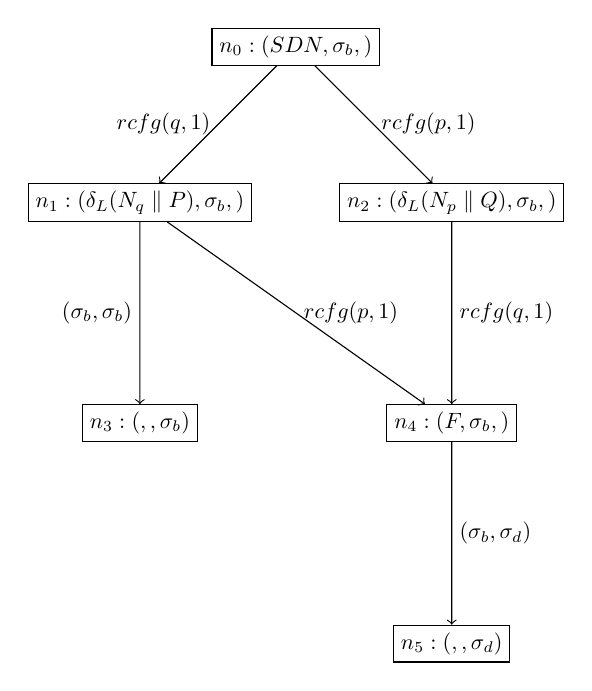
\begin{tikzpicture}[node distance={35mm},
                scale=0.8,
                s/.style = {draw, rectangle,minimum width=5mm,transform shape} ]
            \node[s] (n0) {$n_0: (SDN,\sigma_b,\his{})$};
            \node[s] (n1) [below left of=n0]
            {$n_1: (\delta_{\mc{L}}(N_q \parallel P),\sigma_b,\his{})$};
            \node[s] (n3) [below of=n1]
            {$n_3: (\checkmark,\his{},\sigma_b)$};
            \node[s] (n2) [below right of=n0]
            {$n_2: (\delta_{\mc{L}}(N_p \parallel Q),\sigma_b,
                    \his{})$};
            \node[s] (n4) [below of=n2]
            {$n_4:(F,\sigma_b,\his)$};
            \node[s] (n5) [below of=n4]
            {$n_5:(\checkmark,\his{},\sigma_d)$};
            \draw[->,s] (n0) -- node[left]{$rcfg(q,1)$} (n1);
            \draw[->,s] (n0) -- node[right]{$rcfg(p,1)$} (n2);
            \draw[->,s] (n1) -- node[left]{$(\sigma_b,\sigma_b)$} (n3);
            \draw[->,s] (n1) -- node[right]{$rcfg(p,1)$} (n4);
            \draw[->,s] (n2) -- node[right]{$rcfg(q,1)$} (n4);
            \draw[->,s] (n4) -- node[right]{$(\sigma_b,\sigma_d)$} (n5);
        \end{tikzpicture}
    \end{figure}
\end{frame}

\begin{frame}{Example: Loop Freedom}
    \begin{center}
        \begin{tikzpicture}[node distance={20mm},main/.style = {draw, circle,minimum size=8mm}]
            \node[main] (a)  {$a$};
            \node[main] (b) [above of=a]  {$b$};
            \node[main] (c) [left of=b] {$c$};
            \node[main] (d)  [below of=c] {$d$};
            \draw [->,green,thick] (a) -- (b);
            \draw [->,green,thick] (b) -- (c);
            \draw [->,orange,thick] (c) -- (d);
            \draw [->,green,thick,dashed] (a) -- (c);
            \draw [->,orange,thick,dashed] (c) edge[bend left] (b);
            \draw [->,orange,thick,dashed] (b) -- (d);
            \draw pic["$p$",
            draw=blue,->,thick,angle eccentricity=1.2,
            angle radius=1.2cm] {angle=b--a--c} ;
            \draw pic["$q$",
            draw=blue,<-,thick,angle eccentricity=1.2,
            angle radius=0.8cm] {angle=b--c--d} ;
        \end{tikzpicture}
    \end{center}

    Events:
    \begin{align*}
        l(p_1) = l(p_2) & = rcfg_{p,1}  \\
        l(q_1) = l(q_2) & = rcfg_{q,1} \\
        l(bb) & = b \ra b \\
        l(cc) & = c \ra c \\
    \end{align*}
\end{frame}

\begin{frame}{Example: Loop Freedom}
    Property: Loop Freedom
    \begin{align*}
        \f{PV} = \exists c \in \mc{F}(ES(\vec v)).
        l(c) = \alpha\cdot\pi \Rightarrow \alpha(sw) = \pi(sw)
    \end{align*}
    \begin{center}
        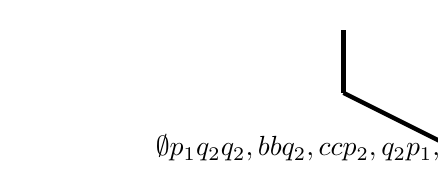
\begin{tikzpicture}[scale=0.8]
            \crd{0}{0}{$\emptyset$}
            \crd[below]{-2}{1}{$\s{p_1}$}
            \crd[below]{2}{1}{$\s{q_2}$}
            \crd[above]{2}{2}{$\s{q_2,bb}$}
            \crd[above]{4}{2}{$\s{q_2,cc}$}
            \crd[above]{0}{2}{$\s{p_2,q_2}$}
            \crd[left]{-2}{2}{$\s{p_1,q_1}$}
            \draw [ultra thick] (0,0) -- (2,1);
            \draw [ultra thick] (0,0) -- (-2,1);
            \draw [ultra thick] (2,1) -- (0,2);
            \draw [ultra thick] (2,1) -- (2,2);
            \draw [ultra thick] (2,1) -- (4,2);
            \draw [ultra thick] (-2,1) -- (-2,2);
        \end{tikzpicture}
    \end{center}
    Is $M_{\s{p_2},q_2} = \F$ a cause of $PV = \T$?
    \begin{equation*}
        M_{\s{p_2},q_2} = \T \iff \s{p_2} \vdash_{min} q_2 
        \ (\text{in } ES(\vec v))
    \end{equation*}
\end{frame}

\begin{frame}{Example: Loop Freedom}
    \begin{align*}
        \f{M_{\e,q_2}}  & = Min(\e,q_2) \wedge Con(\e) \\
                        & = Min(\e,q_2)                \\
                        & =  \bigwedge_{q_2 \notin s'}
        \neg M_{s',q_2}                                \\
        \f{EN_{\e,q_2}} & = M_{\e,q_2}
    \end{align*}
    \begin{equation*}
        M \vDash [M_{\s{p_2},q_2} \la \T] M_{\e,q_2} = \F \wedge
        EN_{\e,q_2} = \F
    \end{equation*}
    \begin{center}
        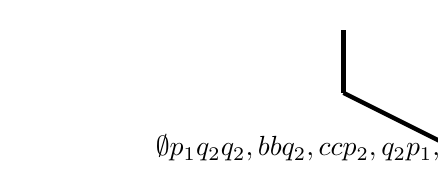
\begin{tikzpicture}[scale=0.8]
            \crd{0}{0}{$\emptyset$}
            \crd[below]{-2}{1}{$\s{p_1}$}
            \crd[below]{2}{1}{$\s{q_2}$}
            \crd[above]{2}{2}{$\s{q_2,bb}$}
            \crd[above]{4}{2}{$\s{q_2,cc}$}
            \crd[above]{0}{2}{$\s{p_2,q_2}$}
            \crd[left]{-2}{2}{$\s{p_1,q_1}$}
            \draw [ultra thick] (0,0) -- (2,1);
            \draw [ultra thick] (0,0) -- (-2,1);
            \draw [ultra thick] (2,1) -- (0,2);
            \draw [ultra thick] (2,1) -- (2,2);
            \draw [ultra thick] (2,1) -- (4,2);
            \draw [ultra thick] (-2,1) -- (-2,2);
        \end{tikzpicture}
    \end{center}
\end{frame}